% TODOP: Dodaj odpowienie artefakty latexa go .gitignore
\documentclass[11pt,a4paper]{article}

\usepackage[T1]{fontenc}
\usepackage[utf8]{inputenc}
\usepackage[polish]{babel}
\usepackage{lmodern}
\usepackage{microtype}
\usepackage[margin=2.4cm]{geometry}

\usepackage{graphicx}
\usepackage{booktabs}
\usepackage{rotating}
\usepackage{array}
\usepackage{xcolor}
\usepackage{listings}
\usepackage[font=small,labelfont=bf]{caption}

\usepackage{pgfplots}
\pgfplotsset{compat=1.18}
\usepgfplotslibrary{groupplots}

\usepackage[backend=bibtex,style=numeric,sorting=none]{biblatex}
\addbibresource{refs.bib}

\usepackage[hidelinks]{hyperref}

\newcommand{\todo}[1]{\textcolor{red}{\textbf{[DO UZUPEŁNIENIA: #1]}}}
\newcommand{\dopisz}{\textcolor{red}{\textbf{[DO UZUPEŁNIENIA]}}}

\lstset{
  basicstyle=\ttfamily\footnotesize,
  keywordstyle=\bfseries,
  commentstyle=\itshape\color{gray!80!black},
  language=C++,
  columns=fullflexible,
  breaklines=true,
  frame=single,
  framesep=4pt,
  xleftmargin=6pt,
  captionpos=b,
  literate={ą}{{\k{a}}}1 {ć}{{\'c}}1 {ę}{{\k{e}}}1 {ł}{{\l}}1 {ń}{{\'n}}1
           {ó}{{\'o}}1 {ś}{{\'s}}1 {ź}{{\'z}}1 {ż}{{\.z}}1
}

\title{\vspace{-1.2cm}Porównanie modeli równoległych obliczeń inkrementalnych\\
       PSAC i Query w zastosowaniu do kompilatorów}
\author{Piotr Oleszczuk \and Piotr Trzaskowski \and Jakub Bartmiński} % TODOP: Ustaw alfabetycznie
\date{Projekt Badawczy, rok akademicki 2025/2026\\
      Wydział Matematyki, Informatyki i Mechaniki\\
      Uniwersytet Warszawski\\[2pt]
      Opiekun: Aleksy Schubert}

\begin{document}
\maketitle

\begin{abstract}
Kompilator inkrementalny musi jednocześnie korzystać z wielu rdzeni i szybko % TODOP: Wspóbieżny kompilator inkremantalny. Sam inkrementalny nie musi
przeliczać wynik po drobnej edycji kodu. Porównaliśmy dwa modele obliczeń, które
dają obie te rzeczy naraz: PSAC (\emph{Parallel Self-Adjusting Computation}),
oparty na propagacji zmian po zapisanym śladzie wykonania, oraz Query, autorski
framework zapytań zespołu duckling, oparty na grafie zapytań z cache'em wyników. % Używany przez język Duckling, rozwijany przez firme DuckType.
Napisaliśmy dwa mikrobenchmarki, każdy celowo dopasowany do innego modelu, oraz
dwa pełne kompilatory inkrementalne, które dzielą ten sam front end i ten sam
generator kodu, a różnią się wyłącznie silnikiem inkrementalnym. Mikrobenchmarki
dały wyraźny wynik: PSAC jest do 17 razy szybszy przy płytkich zależnościach
drzewiastych, a Query do 2,5 raza szybsze przy gęstych zależnościach
współdzielonych. W prawdziwym kompilatorze ta przewaga w dużej mierze zniknęła:
różnice między silnikami zmieściły się w 5--20\% na zimno i były nieistotne na % TODOP: Sformuowania na ciepło, na zimno sa troche dziwne. mozna je jakos podmienic?
ciepło. Zamiast tego o czasie przebudowy zdecydowała granularność śledzonych
zależności, której poprawa dała efekt o rząd wielkości większy niż jakakolwiek
różnica między silnikami. Wnioski wykorzystaliśmy do optymalizacji produkcyjnego % TODOP: Produkcyjnego kompilatora Duckling
kompilatora, gdzie zmiana alokatora pamięci i usunięcie globalnej blokady dały % TODOP: Jakiej globalnej blokady. Dopisz
odpowiednio do 50\% i 10--20\% przyspieszenia.
\end{abstract}

\section{Wprowadzenie i pytania badawcze}

Od kompilacji dużego projektu oczekuje się dziś dwóch rzeczy naraz. Po pierwsze,
ma korzystać ze wszystkich dostępnych rdzeni, bo czas pełnej kompilacji przekłada
się wprost na koszt integracji ciągłej. Po drugie, ma reagować na pojedynczą
edycję tak szybko, żeby wydawało się to natychmiastowe, bo z tego samego potoku
korzysta serwer języka obsługujący edytor. Te wymagania nie są niezależne:
zrównoleglenie opłaca się tylko wtedy, gdy jest co liczyć, a inkrementalność ma
sens tylko wtedy, gdy ponowne użycie wyników nie kosztuje więcej niż samo
policzenie ich od nowa.

Są dwa znane podejścia do tego problemu. Pierwsze to \emph{self-adjusting
computation}: program wykonuje się raz i zapisuje ślad swojego wykonania wraz
z informacją o tym, które dane wejściowe czytał. Po zmianie wejścia system
przepycha tę zmianę przez ślad i wykonuje ponownie tylko te fragmenty, które od
niej zależą. Model PSAC~\cite{psac2021} rozszerza to na programy równoległe
i układa ślad w drzewo szeregowo-równoległe. Drugie podejście to \emph{grafy
zapytań}: obliczenie dzieli się na nazwane, czyste zapytania, których wyniki
trafiają do cache'u, a zależności odkrywane są w trakcie wykonania. Do tej grupy
należy Query, framework używany w produkcyjnym kompilatorze języka Duckling. % TODOP: usuń to słowo produkcyjny, stad i z innych miejsc
Autorska jest przy tym konkretna implementacja tego frameworka, a nie sam pomysł
grafu zapytań z cache'em.

Pytanie, które postawiliśmy sobie na początku, brzmiało prosto: który z tych
dwóch modeli lepiej nadaje się na silnik kompilatora inkrementalnego? Rozbiliśmy
je na cztery pytania badawcze:

\begin{description}
  \item[RQ1] Który silnik ma mniejszy narzut własny, w oderwaniu od realnej pracy?
  \item[RQ2] Jak oba skalują się wraz z liczbą wątków?
  \item[RQ3] Czy przewaga zmierzona na mikrobenchmarkach przenosi się na
        prawdziwy kompilator?
  \item[RQ4] Co bardziej decyduje o czasie przebudowy inkrementalnej: wybór
        silnika czy granularność śledzonych zależności?
\end{description}

Odpowiedzi zbieramy w sekcjach~\ref{sec:dyskusja} i~\ref{sec:wnioski}. % TODOP: Usuń te linię

\section{Dwa modele obliczeń inkrementalnych}
\label{sec:modele}

\paragraph{PSAC.} Program w modelu PSAC czyta dane wejściowe wyłącznie przez
specjalne, modyfikowalne komórki. Każdy odczyt komórki tworzy w śladzie wykonania
węzeł odczytu, a każde rozwidlenie równoległe tworzy węzeł równoległy, dzięki
czemu ślad ma postać drzewa szeregowo-równoległego. To drzewo nie jest tylko
planem wykonania, ale też zapisaną strukturą zależności. Zapis nowej wartości do
komórki oznacza jako nieaktualne te węzły odczytu, które ją czytały. Propagacja
przechodzi drzewo i wykonuje ponownie tylko nieaktualne poddrzewa, rozwidlając
się przy tym tak samo jak wykonanie pierwotne. Wykonaniem steruje scheduler
fork-join z kradzieżą zadań (work stealing): każde rozwidlenie odkłada jedną
gałąź na lokalną kolejkę wątku, a wolne wątki podbierają pracę z kolejek losowo
wybranych sąsiadów, więc jedna kosztowna gałąź nie blokuje reszty. PSAC nie
zapamiętuje jednak wyników po tym, co dane podobliczenie liczy. Jeżeli dwa różne
miejsca programu liczą to samo, praca wykona się dwa razy.

\paragraph{Query.} W modelu Query obliczenie dzieli się na zapytania, z których
każde ma swój klucz. Wynik zapytania trafia do cache'u, więc dwa niezależne
zapytania o ten sam klucz wykonają pracę tylko raz. Zależności deklaruje się
w trakcie wykonania: funkcja obsługująca zapytanie odpytuje \emph{side inputy},
czyli liście grafu, których kluczem jest sama wartość wejściowa. Po zmianie
wejścia stary liść znika z grafu, a framework przechodzi graf zależności
w odwrotnym kierunku i kasuje dokładnie te węzły, które od niego zależały.
Ponowne wykonanie następuje dopiero przy kolejnym odpytaniu. Za równoległość
odpowiada pula zadań, która wykonuje niezależne zapytania jednocześnie.

Różnice zbiera tabela~\ref{tab:modele}. Z punktu widzenia kompilatora
najważniejsze są dwie: obecność cache'u wyników oraz to, że w PSAC struktura
równoległości i struktura zależności to jedno i to samo drzewo.

\begin{table}[htbp]
\centering
\caption{Porównanie modeli PSAC i Query.}
\label{tab:modele}
\small
\begin{tabular}{@{}p{3.2cm}p{5.4cm}p{5.4cm}@{}}
\toprule
\textbf{Cecha} & \textbf{PSAC} & \textbf{Query} \\
\midrule
Kierunek wykonania
  & przepychanie zmiany (push)
  & wykonanie na żądanie (pull) \\
Struktura ponownego użycia
  & zapisany ślad wykonania w postaci drzewa szeregowo-równoległego
  & graf zapytań z cache'em wyników \\
Jednostka ponownego użycia
  & węzeł odczytu w śladzie
  & zapytanie o danym kluczu \\
Deklaracja zależności
  & odczyt modyfikowalnej komórki wewnątrz zakresu dynamicznego
  & odpytanie side inputu \\
Reakcja na zmianę wejścia
  & zapis unieważnia czytelników, propagacja przechodzi nieaktualne poddrzewa
  & unieważnienie po odwrotnym grafie zależności, przeliczenie na żądanie \\
Współdzielone podobliczenia
  & brak cache'u, praca może się dublować
  & cache gwarantuje jednokrotne wykonanie \\
Model równoległości
  & fork-join z kradzieżą zadań, ślad jest zarazem planem wykonania
  & pula zadań, zapytania zlecane jako punkty wejścia \\
Nieudane podobliczenie
  & zależność od hasha całego programu
  & zależność od hasha całego programu \\
\bottomrule
\end{tabular}
\end{table}

\section{Metodologia}
\label{sec:metodologia}

Eksperyment prowadziliśmy na dwóch poziomach.

\paragraph{Poziom pierwszy: mikrobenchmarki.} Napisaliśmy dwa syntetyczne % TODOP: Nie podoba mi sie sformuowanie mikrobenchmarki. Zamień na benchmarki syntetyczne
obliczenia, każde celowo dopasowane do innego modelu, żeby zobaczyć, jak duża
może być przewaga każdego z nich w najlepszym dla niego przypadku.

\emph{ArraySum} to drzewo przedziałowe nad tablicą liczb: wartość węzła jest sumą
wartości jego dzieci, a liśćmi są pojedyncze elementy tablicy. Zależności są tu
płytkie i drzewiaste, a każdy zakres \texttt{[l,r)} występuje dokładnie raz, więc
nie ma współdzielonych poddrzew i cache Query nie ma czego ponownie użyć, wnosi
tylko narzut. Aktualizacja zmienia zadany procent elementów tablicy, a zmiana
propaguje się ścieżką od liścia do korzenia, dotykając logarytmicznie mało
węzłów. To benchmark dopasowany do PSAC.

\emph{DAG} to warstwowy graf skierowany: \(N\) warstw po \(M\) wierzchołków,
krawędzie tylko między sąsiednimi warstwami, a wartość wierzchołka to jego waga
plus suma wartości poprzedników. Zależności są gęste i współdzielone, bo jeden
wierzchołek jest poprzednikiem wielu, więc jego zmiana wpływa na dużą część
grafu. Cache Query sprawia, że każdy wierzchołek liczony jest dokładnie raz,
podczas gdy PSAC wykonuje tu pracę podwójnie. To benchmark dopasowany do Query.

Oba mierzyliśmy w dwóch trybach: samo obliczenie oraz obliczenie wraz
z aktualizacją inkrementalną. Parametrem \emph{workload} sterowaliśmy ilością
sztucznej pracy przypadającej na jeden węzeł. Ten parametr jest kluczowy: przy
wartości zero mierzymy czysty narzut frameworka, a przy wyższych wartościach
narzut rozmywa się w prawdziwej pracy, co odpowiada sytuacji w kompilatorze.

\paragraph{Poziom drugi: prawdziwe kompilatory.} Napisaliśmy dwa kompilatory
inkrementalne dla tego samego podzbioru języka Duckling: funkcje z rekurencją,
podstawowe typy, klasy z polami, tablice w stylu C, przestrzenie nazw, stałe,
zmienne globalne i import wielu plików. Oba kompilują każdą funkcję do osobnego
pliku obiektowego, równolegle, i linkują wynik jednym wywołaniem systemowego
linkera.

Najważniejsze w tym porównaniu jest to, że \emph{psacklinger} i % TODOP: Moze nie byc jasne co to za nazwy. Powiedz ze to te nasze zaimplentowane kompilatory
\emph{querylinger} dzielą cały front end oraz cały generator kodu: ten sam
parser, tę samą rejestrację deklaracji globalnych, te same tablice symboli i to
samo generowanie kodu LLVM. Różnią się wyłącznie tym, jak decydują, co
przekompilować. Dzięki temu każdą zmierzoną różnicę można przypisać silnikowi
inkrementalnemu, a nie jakości implementacji front endu. Jako punkt odniesienia
mierzyliśmy też \emph{duckc}, produkcyjny kompilator Ducklinga, oparty na Query,
ale z własnym, znacznie bogatszym front endem i pełną inkrementalnością na
poziomie drzewa składniowego.

To, że oba kompilatory zachowują się tak samo, potwierdza wspólny zestaw około
108 testów typu end-to-end: każdy kompiluje program pełnym potokiem, uruchamia
powstały plik wykonywalny i sprawdza kod wyjścia. Testy inkrementalne dodatkowo
sprawdzają dokładne liczby przekompilowanych funkcji, więc porównanie
granularności opiera się na zachowaniu, a nie na deklaracjach. % TODOP: Przeformuuj. Dziwnie brzmi to zdanie

Listingi~\ref{lst:psac} i~\ref{lst:query} pokazują, jak w obu implementacjach % TODOP: Nie nazywaj tego Listingi to jakies super dziwne. Nie ma bardziej polskiej nazwy?
deklarowana jest zależność.
% TODOP: Daj jakieś kolorowanie składni C++ tu i nizej. Wywal moze całe te listingi. Nikt nie jest w stanie powiedziec co tu w sumie sie dzieje
\begin{lstlisting}[caption={Kompilacja jednej funkcji jako obliczenie PSAC.
Zakres dynamiczny zbiera komórki odczytane w trakcie wykonania, więc zbiór
zależności wyliczany jest od nowa przy każdym przebiegu.},label={lst:psac}]
psac_function(compileUnitPsac, State* s, FunctionUnit* unit, std::string link_name) {
    psac_dynamic_context({
        _psac_context_mods.push_back(&unit->body_mod);
        _psac_context_mods.push_back(&s->structural_mod);
        DynamicDepRecorder recorder(_psac_context_mods, *s, s->ctx);
        compileOneFunction(s->ctx, item, unit->object_path, &recorder);
    });
}
\end{lstlisting}

\begin{lstlisting}[caption={Rejestracja zależności w wersji Query. Obserwator
wywoływany jest w miejscu użycia symbolu, więc funkcja zależy dokładnie od tych
sygnatur, stałych, klas i zmiennych globalnych, których naprawdę użyła.},
label={lst:query}]
DECLARE_QUERY_SIDE_INPUT(SigInput, HashInputKey);

void SymbolUseRecorder::onFunctionUse(const sym::Symbol& symbol) override {
    query_ctx.query<SigInput>({ .hash = functionSigInputHash(program_ctx, symbol) });
}
\end{lstlisting}

\paragraph{Środowisko pomiarowe.} Wszystkie pomiary, i mikrobenchmarki, i
kompilatory, wykonaliśmy na tej samej maszynie: procesor Intel Core Ultra 7 165H
(22 procesory logiczne), 63719~MiB pamięci RAM, system Linux 6.19.6-arch1-1,
kompilator g++-15, kompilacja z flagami \texttt{-O3 -DNDEBUG}. Czasy mierzyliśmy
narzędziem \texttt{hyperfine}, które mierzy czas całego procesu, wykonuje
przebiegi rozgrzewające, powtarza pomiar wielokrotnie dla każdego zestawu
parametrów i podaje średnią wraz z odchyleniem standardowym. Mikrobenchmarki
przeszły pełne przeszukiwanie siatki parametrów: 3 przebiegi rozgrzewające
i około 48 powtórzeń na punkt pomiarowy, 384 punkty pomiarowe dla ArraySum i 192
dla DAG. Benchmark kompilatorów używał 5 powtórzeń na wariant. Nie stosowaliśmy
przypisywania wątków do konkretnych rdzeni, wyłączania trybu turbo ani % TODOP: Usuń ostatnie zdanie
wymuszania trybu pracy procesora.

\section{Wyniki: mikrobenchmarki}
\label{sec:mikro}

Siatka parametrów obejmowała tryb (samo obliczenie albo obliczenie
z aktualizacją), procent aktualizowanych wejść (1, 10, 50, 100), workload % TODOP: Powiedz ze to 1, 10, 50, 100 to procenty updateów
(0, 50, 100) oraz liczbę wątków (1, 4, 8, 16). Tablica w ArraySum miała rozmiar % TODOP: i wytłumacz tu jak działa workload i co w ogole oznaczaja te liczby (0, 50, 100)
65536 albo 262144, a graf w DAG-u 50 warstw po 100 wierzchołków i 10000 krawędzi.
Wyniki podajemy jako stosunek średniego czasu Query do średniego czasu PSAC,
więc wartość powyżej jedności oznacza, że PSAC jest szybszy. Pełne wyniki
przedstawiają rysunki~\ref{fig:array} i~\ref{fig:dag}.

\begin{sidewaysfigure}[p]
\centering
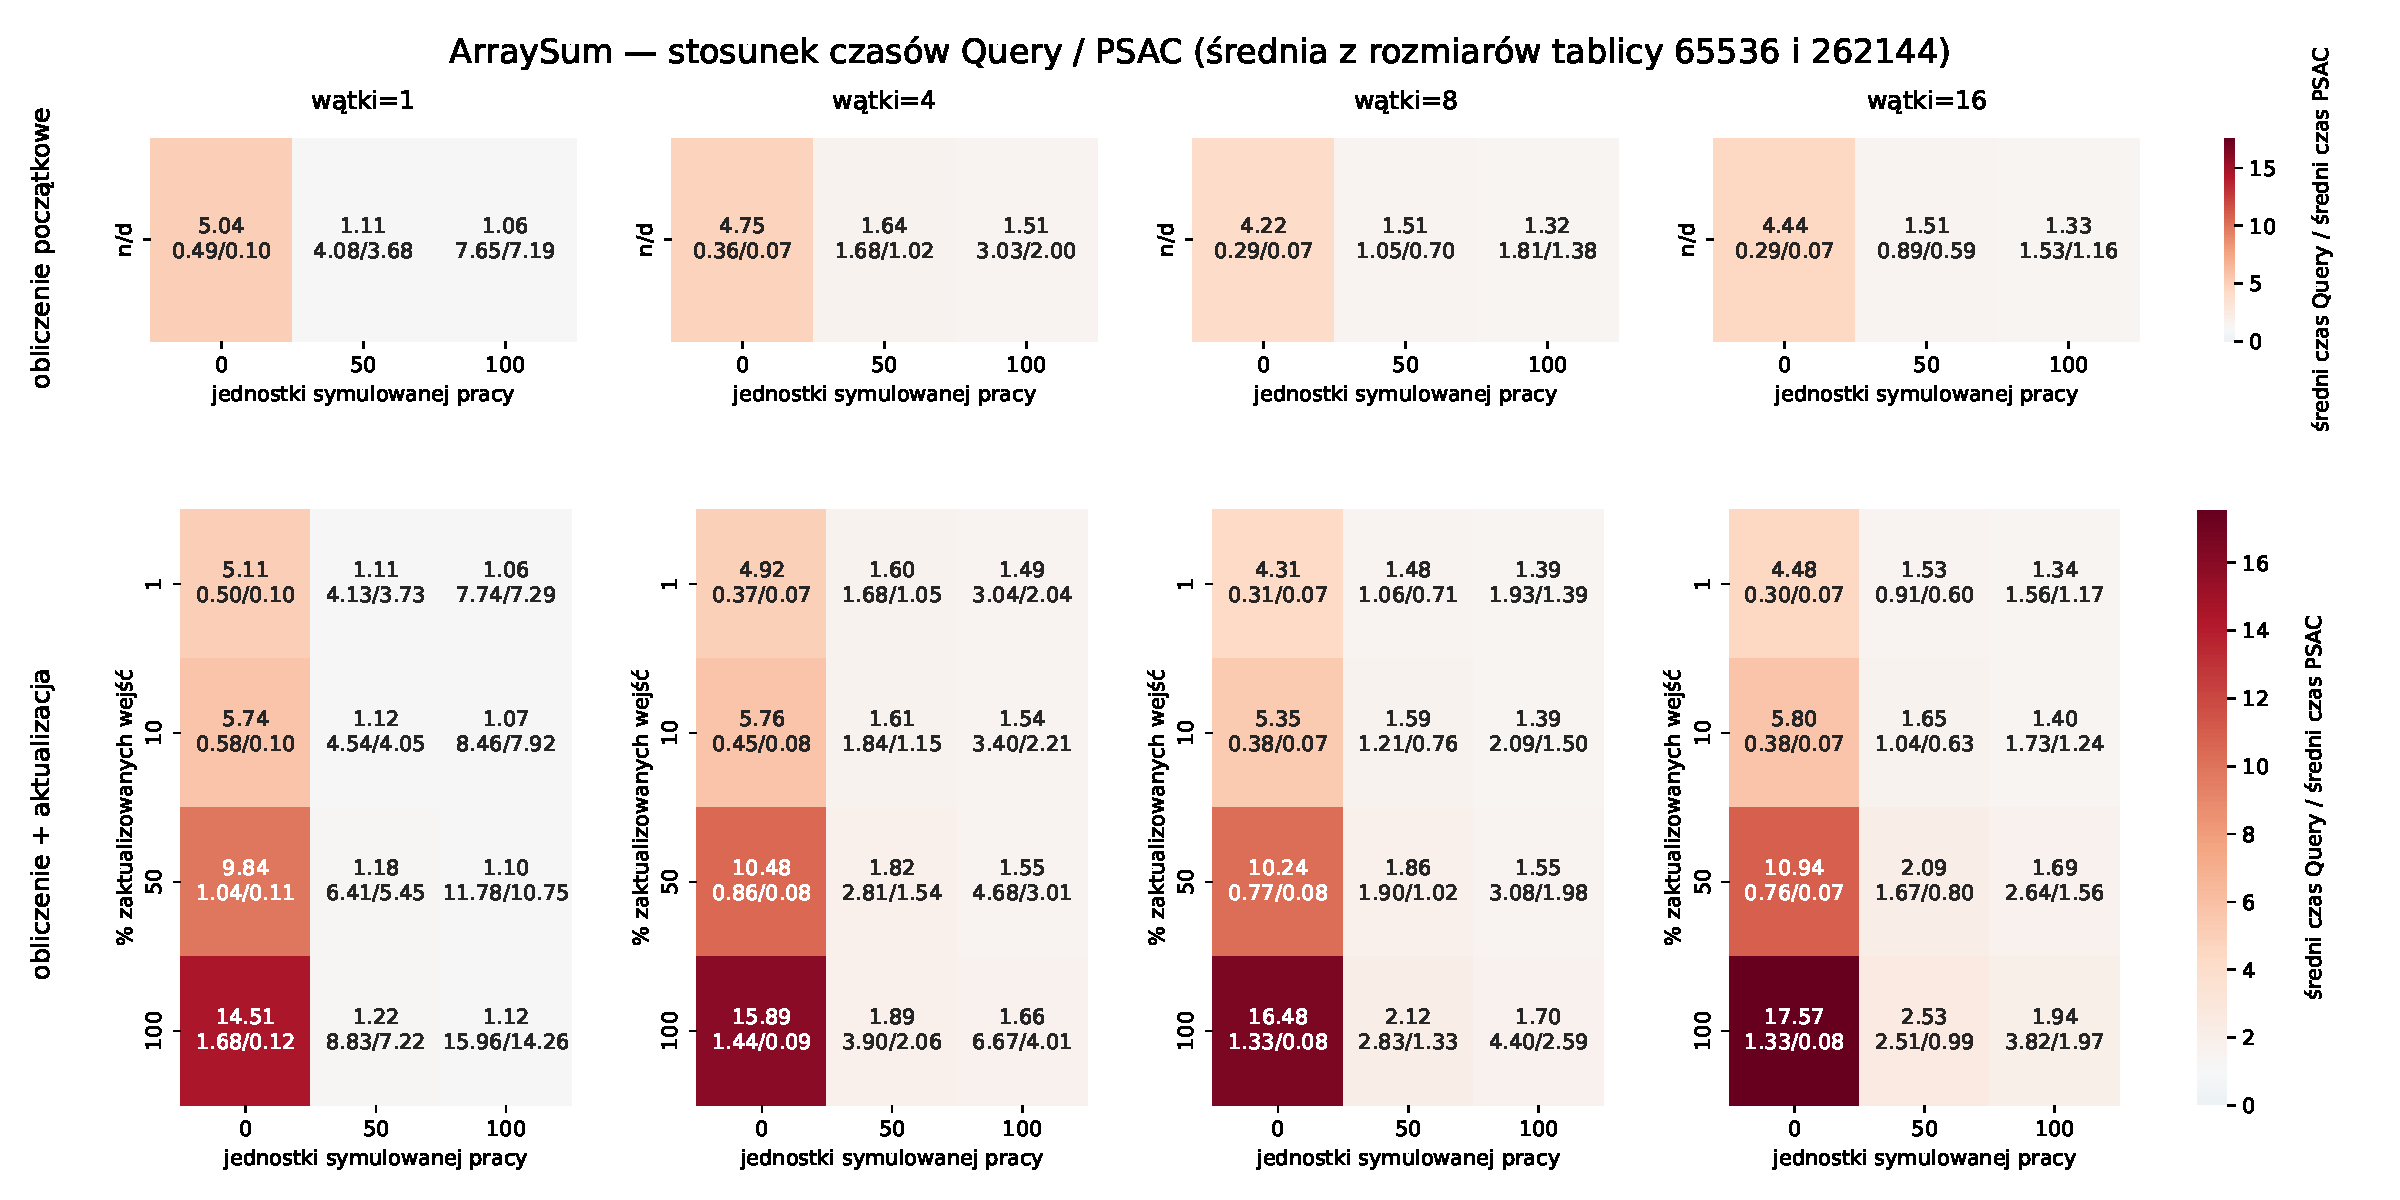
\includegraphics[width=\textheight]{figures/results_array.pdf}
\caption{ArraySum: stosunek średniego czasu Query do średniego czasu PSAC.
Wiersze odpowiadają trybowi pomiaru, kolumny liczbie wątków. W każdej komórce
u góry podany jest stosunek czasów, a pod nim czas Query i czas PSAC w sekundach.
Kolor koduje ten sam stosunek: odcienie czerwieni oznaczają przewagę PSAC-a,
odcienie błękitu przewagę Query, a biel remis. W trybie samego obliczenia oś
procentu aktualizacji zwinęliśmy do jednego wiersza, bo nic się tam nie przelicza
i wszystkie jej wartości są takie same. Wyniki są uśrednione po obu rozmiarach
tablicy.}
\label{fig:array}
\end{sidewaysfigure}

\begin{sidewaysfigure}[p]
\centering
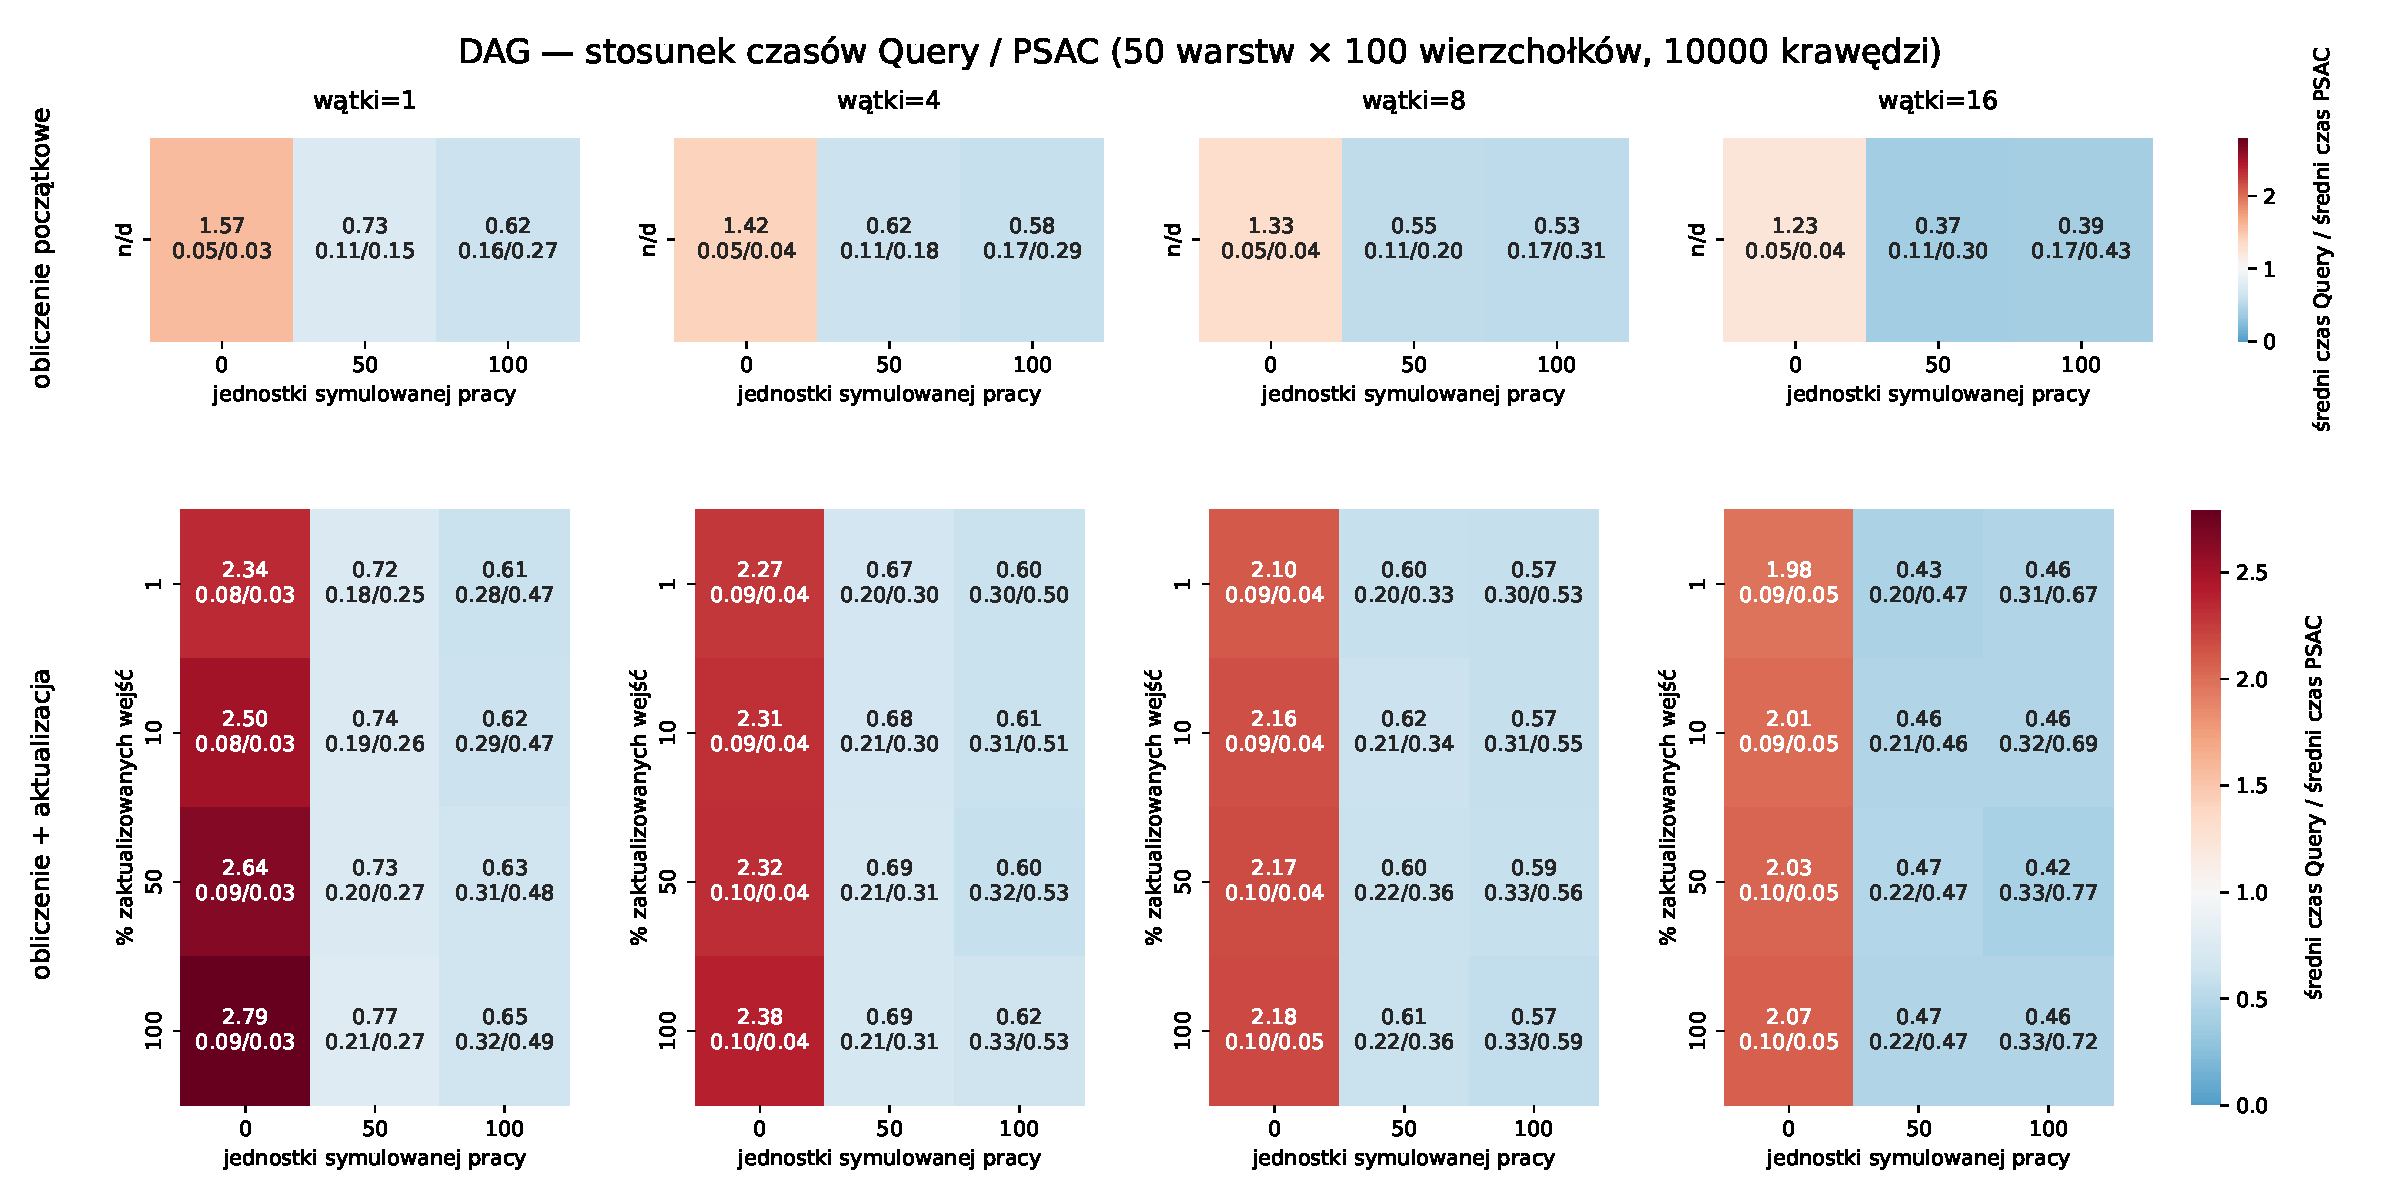
\includegraphics[width=\textheight]{figures/results_dag.pdf}
\caption{DAG: stosunek średniego czasu Query do średniego czasu PSAC. Układ
i sposób odczytu jak na rysunku~\ref{fig:array}. Widać zmianę znaku przewagi wraz
ze wzrostem sztucznej pracy oraz to, że procent aktualizowanych wierzchołków
prawie nie wpływa na wynik.}
\label{fig:dag}
\end{sidewaysfigure}

\paragraph{ArraySum.} Przy zerowym workloadzie, czyli na czystym narzucie
frameworka, Query jest 4--5 razy wolniejsze od PSAC-a: stosunek wynosi 5,04 przy
jednym wątku, 4,75 przy czterech, 4,22 przy ośmiu i 4,44 przy szesnastu.
Maszyneria zapytań kosztuje po prostu więcej niż lekki ślad PSAC-a. Wraz ze
wzrostem sztucznej pracy przewaga maleje: przy workloadzie 50 stosunek mieści się % TODOP: Nie uzywaj słowa maszyneria, mało formalne
w przedziale 1,11--1,64, a przy workloadzie 100 w przedziale 1,06--1,51. Oba
silniki przyspieszają wraz z liczbą wątków.

W trybie z aktualizacją różnica jest znacznie większa. Przy zerowym workloadzie
i jednym procencie zmienionych elementów Query jest około pięć razy wolniejsze
(5,11 przy jednym wątku, 4,48 przy szesnastu), a przy stu procentach zmienionych
elementów już 14--18 razy wolniejsze (14,51 przy jednym wątku, 17,57 przy
szesnastu). Powód widać w liczbach bezwzględnych: propagacja PSAC-a po prostym
drzewie jest prawie darmowa, bo wzrost procentu aktualizacji z 1 do 100 zmienia
jego czas tylko z 0,10~s na 0,12~s, podczas gdy Query przy tej samej zmianie
przechodzi z 0,50~s na 1,68~s. Przy workloadzie 100 wyniki znów się wyrównują
i Query jest wolniejsze 1,12--1,94 raza.

\paragraph{DAG.} Tutaj obraz się odwraca. Na czystym narzucie PSAC dalej jest
lżejszy, ale przewaga jest mała i maleje z liczbą wątków: 1,57 przy jednym
wątku, 1,42 przy czterech, 1,33 przy ośmiu i 1,23 przy szesnastu. Gdy tylko
pojawia się prawdziwa praca, wygrywa Query: przy workloadzie 50 stosunek spada do
0,73--0,37, a przy workloadzie 100 do 0,62--0,39. Odpowiada za to cache: każdy
wierzchołek liczony jest dokładnie raz, podczas gdy PSAC przy bardziej złożonej
strukturze obliczeń robi tę samą pracę wielokrotnie.

Osobno warto spojrzeć na skalowalność. Przy workloadzie 100 czas PSAC-a
\emph{rośnie} z 0,27~s na jednym wątku do 0,43~s na szesnastu, podczas gdy czas
Query zostaje praktycznie płaski, zmieniając się z 0,16~s na 0,17~s. Nasza
hipoteza, której nie sprawdziliśmy pomiarowo, jest taka, że PSAC słabo radzi
sobie z głębokimi zależnościami między danymi: długie łańcuchy zależności
ograniczają dostępną równoległość, a koszt utrzymania drzewa śladu rośnie
szybciej niż zysk z dodatkowych wątków.

W trybie z aktualizacją przy zerowym workloadzie PSAC jest szybszy w stosunku
1,98--2,79, przy czym stosunek ten prawie nie zależy od procentu aktualizacji
(2,34 dla jednego procentu i 2,79 dla stu, przy jednym wątku). Przy workloadzie
50 i 100 przewaga wraca do Query, ze stosunkiem 0,42--0,77. Kontrast z ArraySum
jest wyraźny: w gęstym grafie nawet mała zmiana wejścia unieważnia dużą jego
część, więc oba frameworki i tak muszą przeliczyć sporo, przez co procent
aktualizowanych wejść przestaje mieć znaczenie.

\paragraph{Wniosek cząstkowy.} Dla płytkich i prostych zależności lepszy jest
PSAC. Dla zależności gęstych i złożonych, a więc bardziej podobnych do tego, co
dzieje się w kompilatorze, przewagę ma Query, i to tym wyraźniej, im więcej
wątków i im więcej prawdziwej pracy.

\section{Wyniki: kompilatory}
\label{sec:kompilatory}

Korpusem były dwa pliki wygenerowane automatycznie generatorem kodu, po około
8000 linii każdy. Plik \texttt{duck1} zawiera 352 funkcje, \texttt{duck2} 153
funkcje. \todo{czym dokładnie różnią się duck1 i duck2 poza liczbą funkcji}

\subsection{Kompilacja na zimno}

Wszystkie pomiary robiliśmy na zimno: cache inkrementalny i pliki pośrednie % TODOP: Te szczegoly chyba nie mają znaczenia ze czyścilismy pliki i cache inkrementalny. Mozna pominac
kompilatora \texttt{duckc} czyściliśmy przed każdym przebiegiem. Wyniki zbiera
tabela~\ref{tab:zimne}, a rysunek~\ref{fig:skalowanie} pokazuje je jako krzywe
skalowania.

\begin{table}[htbp]
\centering
\caption{Czas kompilacji na zimno w milisekundach, w zależności od liczby wątków
roboczych. Dla \texttt{duckc} liczba ta oznacza liczbę wątków frameworka zapytań,
dla pozostałych liczbę wątków roboczych kompilatora.}
% TODOP: Dodaj do tabeli jednostke, bo nie wiadomo co to za cyferki
\label{tab:zimne}
\small
\begin{tabular}{@{}r rrr c rrr@{}}
\toprule
& \multicolumn{3}{c}{\textbf{duck1} (352 funkcje)} & &
  \multicolumn{3}{c}{\textbf{duck2} (153 funkcje)} \\
\cmidrule(lr){2-4}\cmidrule(lr){6-8}
\textbf{wątki} & duckc & psacklinger & querylinger & &
                 duckc & psacklinger & querylinger \\
\midrule
1  & 764 & 589 & 545 & & 1164 & 459 & 437 \\
2  & 706 & 417 & 369 & & 1159 & 379 & 360 \\
4  & 618 & 333 & 294 & & 1116 & 345 & 315 \\
8  & 585 & 295 & 254 & & 1057 & 334 & 297 \\
16 & 569 & 284 & \textbf{239} & & 1074 & 335 & \textbf{302} \\
\midrule
\multicolumn{8}{@{}l@{}}{\emph{Punkt odniesienia bez frameworka:}
  duckc jednowątkowo 625 / 1070~ms,
  psacklinger sekwencyjnie 588 / 461~ms.} \\
\bottomrule
\end{tabular}
\end{table}

\begin{figure}[htbp]
\centering
\begin{tikzpicture}
\begin{groupplot}[
  group style={group size=2 by 1, horizontal sep=1.6cm},
  width=0.46\textwidth, height=5.0cm,
  xmode=log, log basis x=2,
  xtick={1,2,4,8,16}, xticklabels={1,2,4,8,16},
  xlabel={liczba wątków}, ylabel={czas [ms]},
  ymin=0, ymax=1250,
  grid=both, grid style={gray!22},
  legend style={font=\scriptsize, at={(0.5,1.42)}, anchor=north, legend columns=3,
                draw=none, fill=none, column sep=6pt},
  tick label style={font=\scriptsize},
  label style={font=\small},
  title style={font=\small},
]
\nextgroupplot[title={duck1 (352 funkcje)}]
\addplot[blue!80!black,thick,mark=*] coordinates {(1,764)(2,706)(4,618)(8,585)(16,569)};
\addplot[red!80!black,thick,mark=square*] coordinates {(1,589)(2,417)(4,333)(8,295)(16,284)};
\addplot[teal!80!black,thick,mark=triangle*] coordinates {(1,545)(2,369)(4,294)(8,254)(16,239)};
\legend{duckc, psacklinger, querylinger}
\nextgroupplot[title={duck2 (153 funkcje)}]
\addplot[blue!80!black,thick,mark=*] coordinates {(1,1164)(2,1159)(4,1116)(8,1057)(16,1074)};
\addplot[red!80!black,thick,mark=square*] coordinates {(1,459)(2,379)(4,345)(8,334)(16,335)};
\addplot[teal!80!black,thick,mark=triangle*] coordinates {(1,437)(2,360)(4,315)(8,297)(16,302)};
\end{groupplot}
\end{tikzpicture}
\caption{Skalowanie czasu kompilacji na zimno wraz z liczbą wątków roboczych,
dla obu plików wejściowych. Oś pozioma w skali logarytmicznej o podstawie~2.}
\label{fig:skalowanie}
\end{figure}

Z liczb wynikają cztery obserwacje.

Po pierwsze, oba nasze kompilatory biją produkcyjny \texttt{duckc} przy każdej
liczbie wątków: około 2,4 raza na \texttt{duck1} i około 3,6 raza na
\texttt{duck2} przy ośmiu wątkach. Powodem jest to, że dzielimy pracę na
pojedyncze funkcje, podczas gdy \texttt{duckc} wykonuje na jednym dużym module
długi, w dużej części szeregowy łańcuch zadań. % TODOP: Co? Jaki szeregowy łańcuch zadań. Trzeba gdzieś wspomniec ze duckc to jest legitny wielki kompilator moloch ktory mma 100 razy wiecej featureów niz te zabawki

Po drugie, querylinger jest szybszy od psacklingera przy każdej liczbie wątków,
o 5--20\%. Pula zadań frameworka Query nie kosztuje przy tej granularności
więcej niż osobne obliczenia PSAC dla każdej funkcji, a dodatkowo do binarki % TODOP: Wywal część po przecinku to nie ma znaczenia
querylingera nie linkuje się nic ze schedulera PSAC-a, więc jego kręcące się
w kółko wątki nie mogą zaburzyć fazy szeregowej.

Po trzecie, \texttt{duckc} prawie nie zyskuje na dodatkowych wątkach.
Znaleźliśmy przyczynę: budowa drzewa składniowego, czyli parsowanie wraz
z liczeniem stabilnych hashy SHA-256 dla każdego elementu, zajmuje około 232~ms
i jest w całości szeregowa, co stanowi mniej więcej połowę czasu przy ośmiu
wątkach. Zrównoleglenie liczenia tych hashy jest tu największą pojedynczą
dźwignią: eksperyment z całkowitym wyłączeniem hashowania skrócił samo
parsowanie z 202~ms do 67~ms.

Po czwarte, rozbicie czasu psacklingera na fazy (\texttt{duck1}, osiem wątków)
pokazuje, gdzie naprawdę schodzi czas: parsowanie 67~ms, rejestracja deklaracji
globalnych 1~ms, zbieranie jednostek pracy wraz z hashowaniem 22~ms, emisja
obiektu ze zmiennymi globalnymi 2~ms, generowanie kodu funkcji 58~ms, linkowanie
55~ms. Faza faktycznie zrównoleglona to więc mniej niż połowa całości, co jest
ważnym kontekstem dla wszystkich powyższych porównań.

Odnotujmy jeszcze jedną obserwację o samym PSAC-u. Jego scheduler tworzy pulę
wątków zanim program wejdzie do funkcji \texttt{main}, a wolne wątki kręcą się
w pętli zamiast spać, przez co szesnaście z nich psuło zawartość pamięci
podręcznej przez całą szeregową fazę front endu. Zatrzymanie puli na jednym wątku
poza fazami równoległymi skróciło pełną kompilację mniej więcej o połowę.

\subsection{Aktualizacje inkrementalne}

Drugi pomiar dotyczy tego, po co w ogóle buduje się silnik inkrementalny: czasu
reakcji na pojedynczą edycję. Kompilatory pracowały w trybie interaktywnym, przy
ośmiu wątkach, a edycje były jednoliniowe. Wyniki zbiera
tabela~\ref{tab:cieple}.

\begin{table}[htbp]
\centering
\caption{Czas aktualizacji inkrementalnej. Podano średni czas w milisekundach
oraz liczbę faktycznie przekompilowanych funkcji.}
\label{tab:cieple}
\small
\begin{tabular}{@{}l cc c cc@{}}
\toprule
& \multicolumn{2}{c}{\textbf{duck1} (352 funkcje)} & &
  \multicolumn{2}{c}{\textbf{duck2} (153 funkcje)} \\
\cmidrule(lr){2-3}\cmidrule(lr){5-6}
\textbf{scenariusz} & psacklinger & querylinger & & psacklinger & querylinger \\
\midrule
brak zmian                    & 109,0 / 0 & 118,4 / 0 & & 107,2 / 0 & 106,4 / 0 \\
edycja ciała funkcji          & 149,8 / 1 & 160,1 / 1 & & 140,0 / 1 & 146,3 / 1 \\
zmiana inicjalizatora globala & 155,9 / 0 & 163,7 / 0 & & 140,2 / 0 & 147,7 / 0 \\
\bottomrule
\end{tabular}
\end{table}

Około 100~ms to podłoga, poniżej której nie da się zejść, bo tyle zajmuje wspólny
front end, który celowo \emph{nie} jest inkrementalny i przy każdej aktualizacji
parsuje oraz analizuje program od nowa. Jest on identyczny w obu kompilatorach
i został zostawiony poza grafem zależności właśnie po to, żeby pomiar dotyczył
samych silników.

Wynik jest jasny, choć nie wskazuje zwycięzcy: przy równej granularności
zależności oba silniki są nie do odróżnienia. Psacklinger jest minimalnie szybszy
na ciepło, querylinger na zimno, a różnice rzędu kilku milisekund mieszczą się
w odchyleniach tego samego rzędu. Nie ogłaszamy tu więc zwycięzcy, bo dane na to % TODOP: Usuń ostatnie zdanie
nie pozwalają.

Warto natomiast zestawić te liczby z historią samego psacklingera. Jego
wcześniejszy, gruboziarnisty silnik przy zmianie inicjalizatora zmiennej % TODOP: Co to w ogole znaczy gruboziarnisty, może usun to 
globalnej przekompilowywał 352 funkcje z 352, w czasie około 220~ms. Przejście na
zależności śledzone dla pojedynczych symboli zbiło ten scenariusz do zera
przekompilowanych funkcji. To zmiana o rząd wielkości większa niż jakakolwiek
różnica, którą zmierzyliśmy między silnikami.

\subsection{Granularność zależności}

Oba silniki doprowadziliśmy do tej samej, sprawdzonej testami granularności.
Zbiera ją tabela~\ref{tab:granularnosc}. Mechanizmy są różne, a wynik ten sam:
w PSAC każdy symbol dostaje własną modyfikowalną komórkę, a w Query własny side
input, przy czym w obu przypadkach zależność zapisywana jest w miejscu, w którym
symbol jest naprawdę używany, przez ten sam wspólny mechanizm obserwatora % TODOP: Nie wiem co to obserwator. Czytelnik tez nie bedzie wiedzial
w generatorze kodu.

\begin{table}[htbp]
\centering
\caption{Granularność zależności. Wyniki identyczne dla obu silników,
potwierdzone testami sprawdzającymi dokładne liczby przekompilowanych funkcji.}
\label{tab:granularnosc}
\small
\begin{tabular}{@{}p{6.4cm}p{7.8cm}@{}}
\toprule
\textbf{Rodzaj edycji} & \textbf{Co zostaje przekompilowane} \\
\midrule
zmiana ciała funkcji & tylko ta funkcja \\
zmiana wartości stałej & tylko funkcje, które ją czytają \\
zmiana inicjalizatora zmiennej globalnej & zero funkcji, tylko ponowna emisja obiektu ze zmiennymi globalnymi i relink \\
zmiana nazwy parametru & tylko ta funkcja, bo hashe sygnatur obejmują typy, a nie nazwy \\
zmiana typu zwracanego & funkcja oraz jej wywołujący, którzy poprawnie zgłaszają błąd typów \\
dodanie pola do klasy & tylko funkcje używające tej klasy \\
dodanie lub usunięcie funkcji & bez pełnej przebudowy, reszta zostaje w cache'u \\
nieudana kompilacja, przyczyna później naprawiona & ponowienie dokładnie tej funkcji, przez zależność od hasha całego programu \\
zmiana importu lub przestrzeni nazw & wszystko, jako bezpieczne rozwiązanie zachowawcze \\
\bottomrule
\end{tabular}
\end{table}

Ostatni wiersz wymaga komentarza. Zmiana importu albo nazwy przestrzeni nazw może
zmienić to, do czego odnosi się dowolna nazwa w programie, więc jedyną poprawną
reakcją jest przekompilowanie wszystkiego. Podobnie zgrubna musi być reakcja na
błąd kompilacji: nieudana kompilacja nigdy nie poznała swojego prawdziwego
zbioru zależności, bo brakujący symbol nie ma jak pojawić się w grafie, więc
jedyne, na czym może się zawiesić, to hash całego programu.

Dodajmy, że hashe treści liczymy z wydruku elementów drzewa składniowego % TODOP: To chyba nie ma znaczenia w tym kontekście
z usuniętymi pozycjami w pliku. Bez tego wstawienie jednej linii przesunęłoby
pozycje wszystkich elementów poniżej edycji i unieważniło je wszystkie.

\section{Optymalizacje produkcyjnego kompilatora}
\label{sec:optymalizacje}

Wnioski z projektu wykorzystaliśmy do optymalizacji produkcyjnego kompilatora
\texttt{duckc}. Wąskie gardła szukaliśmy profilerem \texttt{perf}, nagrywając
przebiegi kompilacji i patrząc, gdzie schodzi czas.

Pierwszą zmianą była zamiana alokatora pamięci na mimalloc. Wpadliśmy na to,
patrząc na konfigurację budowania samego PSAC-a, który go używa: pojawiło się
pytanie, ile z jego lekkości bierze się z modelu obliczeń, a ile po prostu
z tańszych alokacji. Zmiana dała powtarzalne przyspieszenie od 10\% do nawet
50\%. Zużycia pamięci nie zmierzyliśmy.

Po włączeniu mimalloc profil się przesunął i nowym wąskim gardłem okazało się
internowanie napisów, czyli mechanizm, który trzyma jedną kopię każdego
identyfikatora. Chronił go globalny rwlock, przy czym większość czasu schodziła
nie na blokadzie zapisu, ale na blokadzie odczytu na szybkiej ścieżce, czyli
w przypadku, w którym identyfikator już istniał. Zastąpienie tego globalnym
mutexem w połączeniu ze współbieżnymi hashmapami dało 10--20\% w scenariuszu
wielowątkowym. Warto to zapamiętać: blokada odczytu wydaje się tania, ale przy % TODOP: Usuń '' warto to zapamietac
wielu wątkach samo jej zakładanie staje się miejscem, o które wątki się biją.

Trzeci obszar to hashmapy. Używamy własnej implementacji współbieżnej hashmapy
z własnym alokatorem. Sprawdziliśmy alternatywę w postaci Google Swiss Table, ale
w naszym sposobie użycia okazała się wolniejsza. Zmierzyliśmy też, że zły dobór
algorytmu haszującego przy wielu wątkach dodatkowo powoduje przerzucanie linii
pamięci podręcznej między rdzeniami (cache-line bouncing), czyli koszt, którego
w ogóle nie widać w pomiarach jednowątkowych.

Zapisaliśmy też kierunki, których nie zdążyliśmy zrobić: wykrywanie cykli % TODOP: Optymalizacja wykrywania cykli
w grafie zapytań, przyspieszenie haszowania wyników, dalsza walka
z przerzucaniem linii pamięci podręcznej oraz wczytywanie danych z wyprzedzeniem
(software prefetching).

\section{Dyskusja i ograniczenia}
\label{sec:dyskusja}

\paragraph{Mikrobenchmarki a rzeczywistość (RQ3).} Mikrobenchmarki
przewidywały wyraźną przewagę Query na gęstych grafach, sięgającą 2,5 raza przy
prawdziwej pracy. W kompilatorze wyszedł praktycznie remis: querylinger jest
szybszy o 5--20\% na zimno, psacklinger minimalnie szybszy na ciepło.
Przewidywanie sprawdziło się więc co do kierunku, ale nie co do skali. % TODOP: Usuń to zdanie

Naszym zdaniem powód jest taki. Mikrobenchmark z workloadem zero mierzy stosunek
narzutów, ale kompilator nie pracuje w takich warunkach: wygenerowanie kodu
jednej funkcji to milisekundy pracy, wobec których koszt zapisania kilkunastu
zależności jest pomijalny. Do tego duża część czasu leży poza silnikiem
inkrementalnym: w psacklingerze parsowanie i linkowanie to razem około 122~ms
z 295~ms przy ośmiu wątkach. Innymi słowy, mikrobenchmark mierzy dokładnie to,
czego w kompilatorze jest najmniej.

\paragraph{Granularność bije silnik (RQ4).} To jest główny wynik tego projektu.
Przy równej granularności zależności dwa bardzo różne silniki dały wyniki nie do
odróżnienia w granicach błędu pomiaru. Za to zmiana granularności w obrębie
jednego silnika, z gruboziarnistej na śledzenie pojedynczych symboli, zmieniła
jeden ze scenariuszy z 352 przekompilowanych funkcji w 220~ms na zero funkcji.
Wniosek dla projektanta jest więc taki, że przy budowie kompilatora
inkrementalnego wysiłek trzeba kierować najpierw na precyzję śledzenia
zależności i na zmniejszanie tej części pracy, która zostaje poza grafem,
a dopiero potem na wybór silnika.

\paragraph{Kiedy wybór silnika jednak ma znaczenie.} Nie znaczy to, że modele są
wymienne. Przy bardzo lekkich węzłach obliczenia i płytkich zależnościach narzut
Query jest nie do zignorowania, w skrajnym przypadku aż 17-krotny. Przy gęstych
zależnościach i wielu wątkach PSAC przestaje skalować. Kompilator leży akurat
pomiędzy tymi przypadkami, co tłumaczy remis.

\paragraph{Ograniczenia i zagrożenia dla trafności.} Wyniki trzeba czytać
z następującymi zastrzeżeniami:

\begin{itemize}
  \item Mikrobenchmarki są syntetyczne i celowo dopasowane do przeciwnych modeli,
        więc podane stosunki to wartości skrajne, a nie typowe.
  \item Wszystkie pomiary pochodzą z jednej maszyny i jednej serii pomiarowej.
        Nie przypisywaliśmy wątków do konkretnych rdzeni ani nie kontrolowaliśmy
        taktowania procesora, a użyty procesor ma rdzenie o różnej wydajności,
        co przy szesnastu wątkach może zaburzać porównania.
  \item Korpus kompilatorów pochodzi z jednego generatora i obejmuje dwa pliki.
        Nie wiemy, na ile wygenerowany kod przypomina strukturę zależności
        prawdziwego projektu.
  \item Nieinkrementalny front end daje podłogę około 100~ms, która zasłania
        różnice między silnikami w pomiarach na ciepło. Do zmierzonego czasu
        wliczone jest też linkowanie i operacje dyskowe, na które żaden silnik
        nie ma wpływu.
  \item Wyniki ArraySum są uśrednione po dwóch rozmiarach tablicy, rozmiar nie
        jest osobną osią wykresu. Dodatkowo przy zerowym workloadzie wzrost
        procentu aktualizacji z 1 do 100 zmienia czas PSAC-a tylko z 0,10~s na
        0,12~s. Nie udało nam się tego wyjaśnić i nie wykluczamy, że to artefakt
        pomiaru.
  \item Nie zmierzyliśmy zużycia pamięci przez kompilatory, mimo że oba silniki
        mają struktury, które w długiej sesji interaktywnej tylko rosną: tablica
        komórek i wpisy po usuniętych symbolach po stronie PSAC-a, węzły grafu po
        stronie Query.
  \item Nie robiliśmy testów istotności statystycznej. Przy różnicach rzędu kilku
        milisekund i odchyleniach tego samego rzędu to właśnie dlatego świadomie
        nie rozstrzygamy porównania na ciepło.
\end{itemize}

\section{Wnioski i dalsze prace}
\label{sec:wnioski}

Odpowiadając wprost na postawione pytania badawcze:

\textbf{RQ1.} Mniejszy narzut własny ma PSAC. Na czystym narzucie jest lżejszy
w obu mikrobenchmarkach, wyraźnie w ArraySum (4--5 razy) i umiarkowanie
w DAG-u (1,2--1,6 raza).

\textbf{RQ2.} Query skaluje się stabilniej. PSAC skaluje dobrze na płytkim
drzewie ArraySum, ale na gęstym DAG-u jego czas potrafi rosnąć wraz z liczbą
wątków. W kompilatorze oba skalują podobnie i oba wyraźnie lepiej niż
\texttt{duckc}.

\textbf{RQ3.} Tylko częściowo. Kierunek przewagi się zgadza, skala już nie.
Przewidywana przewaga rzędu 2,5 raza skurczyła się do 5--20\% na zimno i do
nieistotnej różnicy na ciepło.

\textbf{RQ4.} Decyduje granularność. Przy równej granularności silniki są nie do
odróżnienia, a poprawa granularności w obrębie jednego silnika dała efekt o rząd
wielkości większy.

Praktyczna rekomendacja dla kompilatora Duckling brzmi więc: zostać przy
frameworku Query, bo jest już zintegrowany z produkcyjnym potokiem i nie kosztuje
mierzalnie więcej przy tej wielkości zadań, a wysiłek kierować na precyzję
zależności i na fazy leżące poza grafem.

Dalsze prace to przede wszystkim: uczynienie front endu inkrementalnym, co
usunęłoby podłogę 100~ms i dopiero wtedy pozwoliłoby uczciwie zmierzyć same
silniki; zrównoleglenie liczenia stabilnych hashy w \texttt{duckc} (eksperyment
wskazał skrócenie parsowania z 202~ms do 67~ms); pomiar zużycia pamięci obu
silników; oraz dokończenie listy z sekcji~\ref{sec:optymalizacje}.

\section{Podział pracy}

\begin{table}[htbp]
\centering
\caption{Podział pracy w projekcie.}
\label{tab:podzial}
\small
\begin{tabular}{@{}p{3.6cm}p{6.4cm}p{4.2cm}@{}}
\toprule
\textbf{Osoba} & \textbf{Obszar odpowiedzialności} & \textbf{Wkład} \\
\midrule
Piotr Oleszczuk    & \dopisz & \dopisz \\
Piotr Trzaskowski  & \dopisz & \dopisz \\
Jakub Bartmiński   & \dopisz & \dopisz \\
\bottomrule
\end{tabular}
\end{table}

\printbibliography[title={Bibliografia}]

\end{document}
